% !TEX TS-program = XeLaTeX
% use the following command: 
% all document files must be coded in UTF-8
\documentclass[french]{textolivre}
% See more information on the repository: https://github.com/leolca/textolivre

% Metadata
\begin{filecontents*}[overwrite]{article.xmpdata}
    \Title{Les stratégies de la post-édition de la traduction automatique des proverbes par des apprenants FLE et de traduction}
    \Author{Rana Kandeel}
    \Language{fr}
    \Keywords{Stratégies \sep Proverbes \sep Traduction automatique \sep Français langue étrangère \sep Post-édition}
    \Journaltitle{Texto Livre}
    \Journalnumber{1983-3652}
    \Volume{14}
    \Issue{3}
    \Firstpage{1}
    \Lastpage{16}
    \Doi{10.35699/1983-3652.2021.29459}

    \setRGBcolorprofile{sRGB_IEC61966-2-1_black_scaled.icc}
            {sRGB_IEC61966-2-1_black_scaled}
            {sRGB IEC61966 v2.1 with black scaling}
            {http://www.color.org}
\end{filecontents*}

\journalname{Texto Livre}
\thevolume{14}
\thenumber{3}
\theyear{2021}
\receiveddate{\DTMdisplaydate{2021}{2}{15}{-1}} % YYYY MM DD
\accepteddate{\DTMdisplaydate{2021}{4}{24}{-1}}
\publisheddate{\DTMdisplaydate{2021}{8}{13}{-1}}
% Corresponding author
\corrauthor{Rana Kandeel}
% DOI
\articledoi{10.35699/1983-3652.2021.29459}
%\articleid{NNNN} % if the article ID is not the last 5 numbers of its DOI, provide it using \articleid{} commmand
% Abbreviated author list for the running footer
\runningauthor{Kandeel}
%\editorname{Daniervelin Pereira}
\sectioneditorname{Daniervelin Pereira}
\layouteditorname{Daniervelin Pereira}

\title{Les stratégies de la post-édition en traduction automatique des proverbes par des apprenants FLE et de traduction}
\othertitle{Estratégias de pós-edição na tradução automática de provérbios por alunos da FLE e da tradução}
\othertitle{Post-editing strategies in automatic translation of proverbs by FFL and translation learners}
% if there is a third language title, add here:
%\othertitle{Artikelvorlage zur Einreichung beim Texto Livre Journal}

\author[1]{Rana Kandeel \orcid{0000-0002-8523-4169} \thanks{Email: \url{RHKandeel@pnu.edu.sa}}}
\affil[1]{Translation Department, College of Languages, Princess Nourah Bint Abdulrahman University, Riyadh, Saudi-Arabia.}

\addbibresource{article.bib}
% use biber instead of bibtex
% $ biber tl-article-template

% set language of the article
\setdefaultlanguage{french}
\setotherlanguage{portuguese}
\setotherlanguage{english}
\setotherlanguage{arabic}
\newfontfamily\arabicfont[Script=Arabic]{Amiri} 
\newfontfamily\arabicfontsf[Script=Arabic]{Amiri}
\newfontfamily\arabicfonttt[Script=Arabic]{Amiri}

% for spanish, use:
%\setdefaultlanguage{spanish}
%\gappto\captionsspanish{\renewcommand{\tablename}{Tabla}} % use 'Tabla' instead of 'Cuadro'
%\AfterEndPreamble{\crefname{table}{tabla}{tablas}\Crefname{table}{Tabla}{Tablas}}

% for languages that use special fonts, you must provide the typeface that will be used
% \setotherlanguage{arabic}
% \newfontfamily\arabicfont[Script=Arabic]{Amiri}
% \newfontfamily\arabicfontsf[Script=Arabic]{Amiri}
% \newfontfamily\arabicfonttt[Script=Arabic]{Amiri}
%
% in the article, to add arabic text use: \textlang{arabic}{ ... }

% for russian text we also need to define fonts with support for Cyrillic script
% \usepackage{fontspec}
% \setotherlanguage{russian}
% \newfontfamily\cyrillicfont{Times New Roman}
% \newfontfamily\cyrillicfontsf{Times New Roman}[Script=Cyrillic]
% \newfontfamily\cyrillicfonttt{Times New Roman}[Script=Cyrillic]
%
% in the text use \begin{russian} ... \end{russian}

% to use emoticons in your manuscript
% https://stackoverflow.com/questions/190145/how-to-insert-emoticons-in-latex/57076064
% using font Symbola, which has full support
% the font may be downloaded at:
% https://dn-works.com/ufas/
% add to preamble:
% \newfontfamily\Symbola{Symbola}
% in the text use:
% {\Symbola }

% reference itens in a descriptive list using their labels instead of numbers
% insert the code below in the preambule:
\makeatletter
\let\orgdescriptionlabel\descriptionlabel
\renewcommand*{\descriptionlabel}[1]{%
  \let\orglabel\label
  \let\label\@gobble
  \phantomsection
  \edef\@currentlabel{#1\unskip}%
  \let\label\orglabel
  \orgdescriptionlabel{#1}%
}
\makeatother
%
% in your document, use as illustraded here:
%\begin{description}
%  \item[first\label{itm1}] this is only an example;
%  % ...  add more items
%\end{description}
 

% custom epigraph - BEGIN 
%%% https://tex.stackexchange.com/questions/193178/specific-epigraph-style
\usepackage{epigraph}
\renewcommand\textflush{flushright}
\makeatletter
\newlength\epitextskip
\pretocmd{\@epitext}{\em}{}{}
\apptocmd{\@epitext}{\em}{}{}
\patchcmd{\epigraph}{\@epitext{#1}\\}{\@epitext{#1}\\[\epitextskip]}{}{}
\makeatother
\setlength\epigraphrule{0pt}
\setlength\epitextskip{0.5ex}
\setlength\epigraphwidth{.7\textwidth}
% custom epigraph - END


% if you use multirows in a table, include the multirow package
\usepackage{multirow}

% add line numbers for submission
%\usepackage{lineno}
%\linenumbers

\begin{document}
\maketitle

\begin{polyabstract}
\begin{abstract}
Cette recherche a pour objectif d’analyser les stratégies utilisées dans la post-édition des proverbes traduits automatiquement du français en arabe par des apprenants du Français Langue Étrangère (FLE). Nous présenterons d’abord les fondements théoriques de la traduction automatique des proverbes ainsi que l’état de l’art. L’étude utilise une approche méthodologique mixte. La méthode quantitative comprend un questionnaire distribué sur les étudiantes de FLE pour connaître l’outil de traduction le plus utilisé dans la traduction automatique. La méthode qualitative est axée sur la collecte des données concernant les erreurs de traduction ainsi que sur l’observation directe des stratégies mises en œuvre dans la post-édition de proverbes traduits par \textit{Google Translate}. Les résultats de l’étude montrent que \textit{Google Translate} est l’outil le plus utilisé en traduction et que les erreurs de traduction automatique sont d’ordre syntaxique, lexical, sémantique et stylistique. Les stratégies mises en œuvre dans la post-édition sont variées : découpage des proverbes en unités linguistiques pour la recherche de sens, recours à une langue-pivot (l’anglais), et recherche des équivalents dans des ressources de référence. L’étude conclut que bien que la traduction automatique des proverbes dans les paires de langues éloignées telles que le français et l’arabe semble complexe, \textit{Google Translate} a constitué un outil d’aide à la compréhension des mots constitutifs des proverbes pour des apprenants FLE, ce qui a permis la compréhension du sens des expressions proverbiales, de trouver leurs équivalents et de les post-éditer.

\keywords{Stratégies \sep Proverbes \sep Traduction automatique \sep Français langue étrangère \sep Post-édition}
\end{abstract}

\begin{portuguese}
\begin{abstract}
Essa pesquisa pretende analisar as estratégias usadas na pós-edição de provérbios traduzidos automaticamente do francês para o árabe pelo Francês como Língua Estrangeira (FLE). Apresentaremos primeiro as bases teóricas da tradução automática de provérbios e, em seguida, o estado da arte. O estudo utiliza uma abordagem metodológica mista. O método quantitativo inclui um questionário distribuído aos estudantes de FLE para descobrir a ferramenta de tradução mais usada na tradução automática. O método qualitativo se concentra na coleta de dados sobre erros de tradução, bem como na observação direta das estratégias implementadas na pós-edição de provérbios traduzidos pelo Google Tradutor. Os resultados do estudo mostram que o Google Tradutor é a ferramenta mais usada na tradução e que os erros na tradução automática são sintáticos, léxicos, semânticos e estilísticos. As estratégias implementadas na pós-edição são variadas, como dividir provérbios em unidades linguísticas para a busca de seus significados, usando uma linguagem pivô, o inglês, para conhecer o significado de provérbios e buscar equivalentes em recursos de referência. O estudo conclui que, embora a tradução automática de provérbios em pares de idiomas distantes, como o par franco-árabe, pareça complexa, o Google Tradutor tem sido uma ferramenta para ajudar um aprendiz de FLE a entender o significado de expressões proverbiais, a encontrar seus equivalentes e a pós-editá-los.

\keywords{Estratégias \sep Provérbios \sep Tradução automática \sep Francês como língua estrangeira \sep Pós-edição}
\end{abstract}
\end{portuguese}

\begin{english}
\begin{abstract}
This research aims to analyze the strategies used in the post-editing of proverbs translated automatically from French into Arabic by French as a Foreign Language (FFL) learners. We will first present the theoretical foundations of machine translation of proverbs as well as the state of the art. The study uses a mixed methodological approach. The quantitative method includes a questionnaire distributed for FFL students to find out the most used translation tool in machine translation. The qualitative method focuses on collecting data on translation errors as well as on directly observing the strategies implemented in the post-editing of proverbs translated by Google Translate. The results of the study show that Google Translate is the most widely used tool in translation and that errors in machine translation are syntactic, lexical, semantic, and stylistic. The strategies implemented in the post-edition are varied such as splitting proverbs into linguistic units for the search of their meanings, using a pivot language, namely English to know the meaning of proverbs and searching for equivalents in reference resources. The study concludes that although the automatic translation of proverbs into distant language pairs such as the French-Arabic pair appears complex, Google Translate has been a tool to help an FFL learner to understand the meaning of proverbial expressions, to find their equivalents and to post-edit them.

\keywords{Strategies \sep Proverbs \sep Machine translation \sep French as a foreign language \sep Post-edition}
\end{abstract}
\end{english}

% if there is another abstract, insert it here using the same scheme
\end{polyabstract}


\section{Introduction}\label{sec-intro}
L’expansion de la traduction automatique et le développement des interfaces proposant de plus en plus des traductions utiles dans une large gamme de situations ont engendré un usage récurrent de ce type de traduction par les sociétés, les professionnels et les futurs traducteurs dans les formations universitaires. La traduction automatique permet de traduire sur des supports variés des textes de tout type, généraux ou spécialisés, comme des logiciels, tutoriels, sous-titres de film, modes d’emploi et sites internet. Cette variété de textes et de supports permet aux futurs professionnels d’être exposés à plusieurs facettes de la traduction, qu’elles soient théoriques, technologiques, pratiques ou professionnelles \cite[p.~216]{orlando_training_2019} ainsi qu’à l’acquisition de nouvelles pratiques et compétences. En parallèle, une multitude d’approches didactiques ont été développées pour mettre en œuvre des activités de formation centrées sur l’étudiant, afin de solliciter sa réflexion sur les pratiques et à mieux le préparer en tant que futur professionnel.  Les travaux d’\textcite{hurtado_albir_competence-based_2007, hurtado_albir_acquisition_2015} sur la compétence en traduction, de \textcite{kiraly_project-based_2006, kiraly_growing_2012, kiraly_authentic_2016} et de \textcite{kandeel_development_2019} sur l’apprentissage par projet, ainsi que d’\textcite{hubscher-davidson_reflection_2008} sur les pratiques didactiques de terrain témoignent du dynamisme des recherches dans la formation universitaire et de l’attention portée à la formation des futurs traducteurs. 

À l’heure actuelle, l’utilisation des technologies dans les formations universitaires implique que les enseignants continuent à développer des stratégies efficaces pour enseigner les technologies de la traduction, et enseigner \textit{avec} elles, afin de répondre au besoin de former les étudiants à ces outils \cite[p.~72]{marshman_translation_2012}. Dans notre contexte de formation universitaire en traduction, nous avons remarqué que les étudiantes en licence, apprenants du français langue étrangère (FLE) ont tendance à traduire les phrases ou les textes en utilisant \textit{Google Translate}, sans tenir compte de l’incapacité de cet outil de traduire certaines expressions figées. Dans le but de permettre aux étudiantes de comprendre les limites de la traduction automatique et de développer leurs compétences en matière de post-édition des proverbes, nous avons, au premier semestre de l’année 2018, demandé à trente-deux étudiantes du département de traduction à l’université Princesse Nourah bint Abdulrahman dans le cadre d’un cours facultatif dispensé dans leur formation sur la traduction assistée par ordinateur (TAO), de traduire automatiquement des proverbes français en arabe, d’analyser les erreurs de traduction et de les post-éditer. L’objectif de cette activité était double : sensibiliser les étudiantes aux limites de l’outil à travers l’analyse des erreurs de traduction, et les inciter à mettre en œuvre des stratégies permettant de corriger la traduction proposée et de produire un proverbe équivalent en arabe.  En effet, les expérimentations menées par les étudiants sur leurs propres pratiques, notamment celles qui sont en relation avec les processus cognitifs et les nouvelles technologies, sont considérées comme une pratique favorable au développement des compétences des apprentis-traducteurs \cite[p.~200]{pym_designing_2016}.

Notre problématique s’intéresse à l’identification des stratégies mises en œuvre par les étudiantes dans la post-édition de la traduction automatique des proverbes français. Pour aborder cette problématique, nous avons posé les questions suivantes : quelles sont les erreurs que produit la traduction automatique des proverbes dans la paire de langues français-arabe avec l’utilisation du moteur de traduction \textit{Google Translate}? Quelles sont les stratégies mises en œuvre lors de la post-édition de la traduction des proverbes? 

Dans le domaine de la traduction, les principales branches de la traductologie sont divisées en trois grandes catégories : la traductologie descriptive pure, la traductologie théorique pure et la traductologie appliquée. Cette dernière, caractérisée comme la branche performative de la traductologie \cite[p.~7]{rabadan_applied_2010}, aborde les études concernant la formation, l’aide à la traduction, la politique et la critique de traductions. C’est dans ce champ que notre problématique s’inscrit, plus spécifiquement dans le domaine de la formation des traducteurs.

L’article se divise en deux parties principales : la première concerne les fondements théoriques de la traduction automatique des proverbes ; elle présente l’enjeu de la traduction automatique des proverbes et l’état de la recherche sur la traduction automatique des expressions figées et la post-édition des textes traduits. La deuxième partie concerne l’expérimentation que nous avons menée dans le cadre de l’étude. Nous y présenterons la méthodologie que nous avons appliquée, ainsi que les résultats obtenus, qui feront l’objet d’une discussion.

\section{L’enjeu de la traduction automatique des proverbes}\label{sec-normas}
La traduction automatique implique de substituer l’utilisation de logiciels informatiques au rôle des humains dans le processus de traduction proprement dit l’utilisation de logiciels informatiques. L’expression désigne ainsi des systèmes informatiques responsables de la production de traductions sans ou avec assistance humaine, dont le caractère principal est l’automatisation de tout le processus de la traduction \cite[p.~431]{hutchins_1995}. Dans la traduction automatique (désormais TA), \textcite[p.~77]{poibeau_traduire_2016} fait la distinction entre deux types de systèmes : le premier concerne les systèmes fondés sur les dictionnaires et les règles d’analyse puis de transfert d’une langue à l’autre. Basés sur l’analyse syntaxique des phrases pour décrire les langues visées, ces systèmes travaillent sur les dictionnaires de la langue-source autant que de la langue-cible, ainsi que sur les règles d’analyse de la langue-source et les règles de transfert d’une langue à l’autre. Le deuxième type regroupe les systèmes statistiques qui s’appuient sur des corpus bilingues alignés, où une phrase de la langue-source est alignée avec une phrase de la langue-cible. 

Les systèmes statistiques tendent à repérer les cooccurrences les plus fréquentes entre langue-source et langue-cible, et à en inférer des traductions potentielles au niveau des mots \cite[p.~81]{poibeau_traduire_2016}. Ils permettent de rendre compte des différents sens des mots en fonction des contextes d’usage. Des systèmes statistiques plus récents reposant sur les architectures neuronales jouent un rôle primordial dans la traduction automatique et l’apprentissage incrémental (ou progressif), grâce au processus de la post-édition synchronique \cite[p.~228]{federico_challenges_2018}. Ils sont capables de détecter les associations lexicales dans le cas des collocations et des expressions figées dans la langue-source, et de les mieux restituer dans la langue-cible \cite{bentivogli_neural_2016, burlot_evaluation_2018, isabelle_challenge_2017}. Bien que les systèmes de traduction automatique soient capables d’analyser des corpus composés de milliards de mots et d’en tirer les différentes réalisations de chacun, ils restent moins performants au niveau de l’analyse des expressions figées de la langue arabe car l’ordinateur doit reconnaitre les unités polylexicales et leur attribuer la signification globale correspondante \cite[p.~248]{mejri_figement_2008}. En effet, la traduction des expressions figées exige de créer un milieu culturel, sans lequel la communication ne se fait pas \cite[p.~1]{vaguer_expressions_2011}. Malgré les progrès spectaculaires de la traduction entièrement automatique, c’est encore loin d’être le cas \cite{yvon_les_2019}, notamment pour la traduction des proverbes. 

Le proverbe constitue en effet « une séquence figée, attestée et appartenant à une catégorie linguistique particulière ; il contient des rimes et se présente fréquemment sous une forme binaire, recourt souvent aux métaphores, sa forme et son sens sont complémentaires » \cite[p.~36]{wozniak_peut-traduire_2010}. Dans la traduction automatique des proverbes, les termes traduits ne sont pas toujours équivalents, les métaphores ne sont même pas traduites et les structures employées ne sont pas identiques. Les solutions à ces problèmes ne sont d’ailleurs pas toujours faciles \cite[p.~33]{madec_traduction_nodate} et la constitution de grands programmes de traduction automatique qui résoudraient pour une langue (ou des langues données) tous les problèmes linguistiques (ambiguïtés lexicales, grammaticales, sémantiques, coréférences, métaphores) reste un vœu pieux. De ce fait, l’intervention humaine reste une exigence essentielle pour corriger la traduction des proverbes. 

Ces problèmes issus de la nature même de la TA et de ce type d’expression figée constituent une partie du processus de traduction qui selon \textcite[p.~9]{kussmaul_training_1995} permettent au traducteur d’internaliser des stratégies et des techniques de résolution de problèmes, en particulier dans la phase de la post-édition. Ils exigent du traducteur de faire un effort conscient d’identification de ces problèmes et font advenir une collaboration plus efficace entre l’homme et la machine.

\section{L’état de l’art}\label{sec-conduta}
La littérature en matière d’utilisation de la technologie dans les formations universitaires est abondante, ce qui n’est pas le cas pour le champ de la correction humaine de la traduction automatique des expressions figées, en particulier par des apprentis traducteurs.

Certains auteurs s’intéressent à l’évaluation et la correction humaines de la traduction \cite{blanchon_pour_2007}, car elles permettent de prendre en charge les notions de fluidité ou d’adéquation du texte cible par rapport au texte source sans se contenter de mesurer la qualité du texte traduit en fonction d’une traduction de référence, sur laquelle se fonde la métrique automatisée. Pourtant, les recherches qui s’intéressent à l’évaluation humaine de la traduction des expressions figées sont peu nombreuses, et elles sont encore plus rares dans le cas de la traduction des proverbes. \textcite{vaguer_expressions_2011} a examiné la traduction des constructions verbales semi-figées françaises vers l’anglais et l’espagnol par deux logiciels de TA en libres accès, Systran et Reverso. Les résultats étaient peu satisfaisants au niveau syntaxique, lexical et sémantique, même si les logiciels étaient capables d’identifier certaines locutions. Reverso était capable de reconnaître certaines expressions figées et de les traduire sans toujours pouvoir les traduire de façon bidirectionnelle. Quant à Systran, il n’était pas capable de traduire un bon nombre de lexèmes. Outre l’incapacité des systèmes de traduction automatique à traduire toutes les expressions figées, le problème de la langue candidate à la traduction se pose dans le cadre de la traduction automatique. En effet, l’arabe est une langue qui, à l’instar du japonais ou du chinois, a une morphologie complexe. Sa traduction automatique reste médiocre en comparaison avec l’anglais ou d’autres langues indo-européennes comme le français ou l’espagnol. 

\textcite{poibeau_traduire_2016} met l’accent sur ce point en soulignant que la traduction automatique est plus performante quand il existe une certaine proximité entre la langue-source et la langue-cible, ce qui n’est pas le cas pour des langues éloignées comme l’arabe et le français. \textcite{isabelle_challenge_2017} soulignent pourtant que les difficultés d’ordre syntaxique, lexical et morphosyntaxique caractérisent la TA pour la paire anglais-français.

La composante statistique combinée aux connaissances de nature linguistique poussée doivent être à la base d’un système de traduction automatique dans les langues éloignées afin de rendre possible la bonne traduction de la sémantique dans ces langues et en tenir compte dans le figement. Comme cette solution n’est pas encore mise en place à grande échelle dans la traduction automatique, certains chercheurs ont tenté de trouver des éléments de réponse pour améliorer la qualité de la traduction automatique entre les paires de langues éloignées telles que l’anglais et l’arabe. \textcite{bessou_contribution_2019} a présenté un analyseur morphologique pour la langue arabe et une liste de règles de transfert morphosyntaxique de l’anglais vers l’arabe pour résoudre des problèmes morphosyntaxiques dans la traduction automatique entre ces paires de langues. Pour la traduction des mots et des expressions figées, la traduction directe est utilisée avec une analyse morphologique de chaque mot afin d’en trouver la forme de base et la rechercher dans un dictionnaire électronique pour trouver le mot correspondant dans la langue-cible. Bien que la recherche s’intéresse aux aspects morphosyntaxiques dans l’analyse des mots à traduire, elle montre bien que la recherche du sens du figement se fait selon une analyse fondée sur les règles. Ce type d’analyse se révèle insuffisant pour la traduction d’expressions plus complexes comme les proverbes, et tout particulièrement dans le cas de la paire de langues français-arabe. Malgré l’usage essentiel des proverbes, leur traduction automatique reste problématique en français.

La présente étude met l’accent sur les interventions humaines qui visent à traduire le figement à la suite de leur traduction par \textit{Google Translate}. Il s’agit de développer la réflexion des apprentis-traducteurs sur la traduction automatique des proverbes et de montrer la nécessité de la mise en œuvre d’un processus de relecture, autrement dit de post-édition du texte cible pour corriger les erreurs linguistiques et sémantiques qui caractérisent les résultats de la traduction automatique. En d’autres termes, participer largement à une compréhension de l’activité de traduction. Dans le cas de l’évaluation humaine de la traduction automatique, les chercheurs mettent l’accent sur les activités et les techniques utilisées par les étudiants qui varient selon l’objectif de la post-édition. \textcite{peraldi_traduction_2016} souligne l’importance de l’intervention des étudiants dans la définition des paramètres sur les types d’erreurs dans l’évaluation de l’efficacité d’une approche combinée entre traduction automatique et traduction assistée par ordinateur dans le domaine de la traduction financière, dans le cadre d’un projet de recherche appliquée sollicité par une entreprise spécialisée dans la traduction financière. L’outil de traduction utilisé est Moses et l’évaluation de la traduction a visé la récurrence et les types d’erreurs générées par la traduction automatique. Cependant, cette évaluation a été conduite pour des textes économiques et non pour les expressions figées.

Dans les formations de traduction, les spécialistes mettent en avant l’importance de la formation de traducteurs à la post-édition pour corriger les erreurs, les classifier et produire un texte de qualité dans la langue cible. Beaucoup de recherches ont été menées pour étudier la post-édition de textes produits par traduction automatique pour préparer des experts dans ce domaine \cite{blagodarna_insights_2018}. Certaines recherches se sont focalisées sur l’évaluation de l’effort déployé dans la post-édition \cite{gaspari_perception_2014, koponen_comparing_2012}, ainsi que sur l’intégration de la post-édition dans les programmes d’études et dans l’enseignement et la formation de traducteurs du point de vue de l’enseignant \cite{ginovart_language_2020, guerberof_arenas_machine_2019, flanagan_testing_2014}. Dans leur recherche sur l’inclusion de la post-édition dans les cours de traduction, \textcite{doherty_design_2014} ont décrit un programme qui contient l’évaluation des outils et des résultats de la TA ainsi que le traitement dans la post-édition. L’intervention des étudiants dans une formation de futurs traducteurs de troisième cycle à City University Dublin en 2012 a consisté à noter les résultats de la TA sur la base de leur précision et de leur maîtrise, dans une expérience de conception et d’évaluation d’un programme statistique de traduction automatique. Pour garantir la fiabilité des résultats, chaque résultat est vu par plusieurs étudiants, aucun correcteur ne juge à la fois de la fluidité et de la pertinence pour le même résultat. En expérimentant les pratiques d’évaluation humaine de ces traductions, les étudiants apprennent les meilleures pratiques. L’enseignement de la post-édition aide également les enseignants à mieux comprendre comment les étudiants procèdent pour modifier les traductions automatiques.

Les chercheurs tirent profit de leurs observations en classe ainsi que des écrits réflexifs des étudiants après le cours \cite{koponen_how_2015} pour mettre en évidence les étapes du processus et les techniques utilisées. Savoir comment la post-édition est exécutée aide d’ailleurs à identifier les profils des post-éditeurs et leurs principales caractéristiques. \textcite{blagodarna_insights_2018} a mené une enquête de terrain pour identifier les tendances communes des professionnels dans la post-édition. L’étude montre que la post-édition est utilisée pour les contenus de haute qualité et que ses résultats peuvent être exploités pour donner des informations sur les mesures des programmes de la formation des traducteurs. Selon \textcite{ginovart_language_2020}, la révision de la production bilingue de la TA à post-éditer constitue l’un des trois niveaux supérieurs de la post-édition.

Le passage en revue des recherches portant sur la formation à la post-édition de la traduction automatique montre la variété des objectifs des interventions dans ce processus en focalisant sur différents types de textes généraux et spécialisés. Les objectifs ont été la définition des paramètres de l’évaluation selon une typologie d’erreurs préétablies ou l’évaluation des résultats de la TA. Quand il s’agit d’examiner la TA des expressions figées, c’est d’ailleurs une personne expérimentée (enseignant-traducteur) qui intervient dans l’évaluation des résultats de la traduction. Cependant, à notre connaissance, aucune recherche n’a examiné les stratégies utilisées par des étudiantes pour corriger la TA des proverbes, à cause de la complexité de la traduction de ces derniers. De plus, étant donné l’éloignement des langues française et arabe, la post-édition de proverbes reste une activité rare dans la formation des futurs traducteurs.


\section{Méthodologie}\label{sec-fmt-manuscrito}
Notre méthodologie se décompose en trois étapes : nous avons d’abord utilisé un questionnaire, composé de deux questions, que nous avons distribué pour vérifier si nos premières observations dans les cours concernant l’utilisation des étudiantes de \textit{Google Translate} étaient correctes. Nous avons voulu aussi savoir si cet outil était utilisé par les étudiantes dans la traduction des proverbes. Ce questionnaire a été distribué à trente-deux étudiantes avant de commencer l’expérimentation de la traduction des proverbes. Les questions en sont : «Quels outils en ligne utilisez-vous dans la traduction des textes?» et «À votre avis, quel est l’outil technologique qui peut être utilisé pour traduire les proverbes français en arabe?»

Dans la deuxième étape, nous avons distribué des fiches de collecte des données sur les résultats de la TA des proverbes et l’analyse des erreurs de ces résultats. La troisième étape consiste en l’observation directe des processus et stratégies mis en œuvre par les étudiantes dans la correction des proverbes traduits et qui ont fait l’objet d’une prise de notes. Pour bien identifier les stratégies de la post-édition, nous avons également posé des questions à l’oral dans notre observation. Les questions portent sur ce que les étudiantes mettent en place pour résoudre les problèmes de traduction erronée des proverbes et pour les post-éditer. Nous avons noté les réponses pour pouvoir identifier les stratégies selon chaque proverbe. Cette démarche fut suivie d’une discussion sur la qualité de la TA. La prise des notes a pour objectif de vérifier que nous avons enregistré toutes les stratégies utilisées. 

Les étudiantes ont commencé par utiliser \textit{Google Translate} dans une salle informatique avant de remplir la fiche de traduction et d’analyse des erreurs. Cette fiche contient trois colonnes : dans la première colonne figurent les proverbes à traduire et les deux autres colonnes étaient à remplir par les étudiantes. La deuxième colonne sert à indiquer les erreurs et la troisième à les analyser. La fiche ne contenait pas de typologie d’erreurs préétablie. De plus, les étudiantes n’avaient sous les yeux ni les proverbes en arabe (ou en anglais) qui peuvent constituer une traduction de référence pour les proverbes français dans la correction, ni l’interprétation de ces proverbes français. Le but de l’activité est de les entraîner à trouver les stratégies susceptibles de résoudre ce type de problèmes. 

Les traductions ont été réalisées par trente-deux étudiantes arabophones dont les niveaux linguistiques varient entre A2 et B1 selon le Cadre Européen Commun de Référence pour les Langues (CECRL). Elles sont inscrites en troisième année d’études françaises dans le département de traduction de l’Université Princesse Nourah bint Abdulrahman. Elles ont réalisé les traductions de proverbes dans le cadre du cours « Traduction assistée par ordinateur (TAO) » dans le cadre de leur licence de traduction. Ce cours facultatif a été dispensé au premier semestre de l’année universitaire 2017-2018. L’expérimentation a eu lieu pendant six heures d’enseignement, soit deux séances de cours consécutives. La première séance était consacrée à la traduction des proverbes et l’analyse des erreurs, et la seconde séance à la correction des traductions.

Les proverbes à traduire sont tirés de l’ouvrage bilingue \textit{Dictionnaire des proverbes français}, publié en 2013 à Al Giza en Egypte\footnote{Voir la liste des références.}.% \cite{rossignol_dictionnaire_2013}. 
Nous avons sélectionné sciemment des proverbes soient simples à la construction syntaxique et lexicale facile à saisir pour les étudiantes, c’est-à-dire qui contiennent des mots familiers et des tournures grammaticales déjà abordées en cours de grammaire (verbes pronominaux, pronoms relatifs, conjugaison des verbes, par exemple). Nous avons également tenu à ce que ces proverbes, au nombre de sept (\Cref{tbl01}), aient des équivalents sémantiques en arabe, la langue maternelle des étudiantes. Nous fournissons les transcriptions des mots arabes en caractères latins selon les systèmes de transcription prescrits par l’Institut du monde arabe\footnote{Comment écrire l’arabe en caractères latins ? \url{https://vous-avez-dit-arabe.webdoc.imarabe.org/langue-ecriture/la-langue-arabe-et-sa-transmission/comment-ecrire-l-arabe-en-caracteres-latins}}. Les traductions données par l’auteur du dictionnaire et leur interprétation sont également présentées dans le même tableau mais ne sont pas données aux étudiantes, sachant que plusieurs traductions sont proposées pour certains proverbes. Cette variété n’affecte en rien leur sens, mais elle présente leur traduction selon différents registres de la langue arabe (standard et familier). L’auteur n’a pas donné les interprétations des proverbes trois et sept, et nous les avons recherchées dans d’autres ressources\footnote{Exressio. Fr \url{https://www.expressio.fr/expressions/faire-d-une-pierre-deux-coups} Citations.ouest-france.fr \url{https://citations.ouest-france.fr/citation-miguel-de-cervantes/homme-propose-dieu-dispose-dieu-33806.html}}. 

\begin{table}[htpb]
\caption{Proverbes français avec leur traduction transcrite en arabe et leur interprétation.}
\label{tbl01}
%\begin{minipage}{\textwidth}
\begin{tabularx}{\textwidth}{lp{0.29\textwidth}p{0.29\textwidth}p{0.29\textwidth}}
\toprule
  & Proverbe en français (langue-source) & Traduction du proverbe en arabe (langue-cible) & Interprétation \\
\midrule
1 & Quand on parle du loup, on en voit la queue (p.~49\footnotemark) &
\textlang{arabic}{أذكر الذئب وهيء القضيب} \newline
Odhkor aldhi'b wa hai' alqadib \newline
\textlang{arabic}{جبنا في سيرة القط جه ينط} \newline
Jebna fi sirat elqot geh yenot \newline
\textlang{arabic}{اذكر غائبا يقترب} \newline
Oudhkor ga'ban yaqtareb &
Parle du loup et prépare ton bâton. On utilise ce proverbe quand quelqu’un apparaît alors qu’il était justement le cœur de conversation. Ce proverbe est particulièrement utilisé en cas de médisance \\

2 & Les loups ne se mangent pas entre eux (p.~41) & 
\textlang{arabic}{الذئاب لا يأكل بعضها بعضا} \newline
Al dhi'ab la ya'koulou b'douha b'dan
\textlang{arabic}{الكلاب متعضش في بعضها} \newline
Al kilab ma tou'desh fi b'daha &
Les crapules sont toujours prêtes à s’accorder quand il s’agit de monter un mauvais coup. \\

3 & Faire d’une pierre deux coups (p.~76) & 
\textlang{arabic}{أصاب عصفورين بحجر واحد} \newline 
Assaba asfourain be hajaren wahed \newline
\textlang{arabic}{ضرب حجرا أصاب اثنين} \newline
Daraba hajaran assab ethnin
& Quand quelqu’un, à l’aide d’un seul jet de pierre, arrive à toucher deux cibles différentes \\

4 & Le malheur des uns fait le bonheur des autres (p.~37) &
\textlang{arabic}{} \newline
Masa'ebo qaomen 'nda qaomen fawaido
& Le malheur de quelqu’un a toujours des répercussions directes et qui profitent à d’autres \\

5 & Après la pluie le beau temps (p.~14). &
\textlang{arabic}{إن بعد العسر يسرا} \newline
Ina ba'd al ousr yousra \newline
\textlang{arabic}{بعد الترحة الفرحة} \newline
B'da el tarha el farha \newline
\textlang{arabic}{ولا بد بعد الليل من فجر} \newline
Wa la boudda B'da alayli men fajr \newline
\textlang{arabic}{ولا بد لليل ان ينجلي} \newline
Wa la boudda lelayli an yanjali \newline
\textlang{arabic}{ما بعد الضيق الا الفرج} \newline
Ma b'd ediq 'ila alfaraj
& Les satisfactions, la gaieté finissent par remplacer les désagréments, la tristesse \\

6 & Qui se ressemble s’assemble (p.~51) & 
\textlang{arabic}{الطيور على أشكالها تقع} \newline
'altouyour ala ashkaleha taq
& Les individus dotés de qualités et défauts semblables souvent s’associent ou forment des couples \\

7 & L’homme propose, Dieu dispose (p.~90). &
\textlang{arabic}{العبد في التفكير والرب في التدبير} \newline
Al a'bdo fi tafkir wa allahou fi tadbir
& Dieu, qui sait le mieux, sait ce qui convient bien à chacun. \\

\bottomrule
\end{tabularx}
%\end{minipage}
\source{d’après l’auteur.}
\end{table}
\footnotetext{Le numéro de la page du Dictionnaire de proverbes français où se trouve le proverbe.}


L’observation des stratégies mises en œuvre par les étudiantes lors de l’utilisation de \textit{Google Translate} 
dans la traduction des proverbes est le processus qui va nous conduire à identifier ces stratégies.

\section{Résultats}\label{sec-formato}

\subsection{Questionnaire}\label{sec-formato}

\begin{itemize}
    \item Les outils les plus utilisés dans la traduction
\end{itemize}

Les résultats de la première question dans le questionnaire (\Cref{fig1}) montrent que la majorité des étudiantes (69\%) utilisent \textit{Google Translate}. 
Les étudiantes qui utilisent \textit{Reverso Contexte} sont moins nombreuses (22\%) et celles qui utilisent d’autres moyens sont rares (9\%). Les autres moyens indiqués par les étudiantes comprennent le dictionnaire bilingue Al Maany\footnote{Dictionnaire Almaany \url{https://www.almaany.com/fr/dict/ar-fr/}} et \textit{Reverso Contexte}\footnote{Reverso contexte \url{https://context.reverso.net/traduction/}}. 

\begin{figure}[htbp]
 \centering
 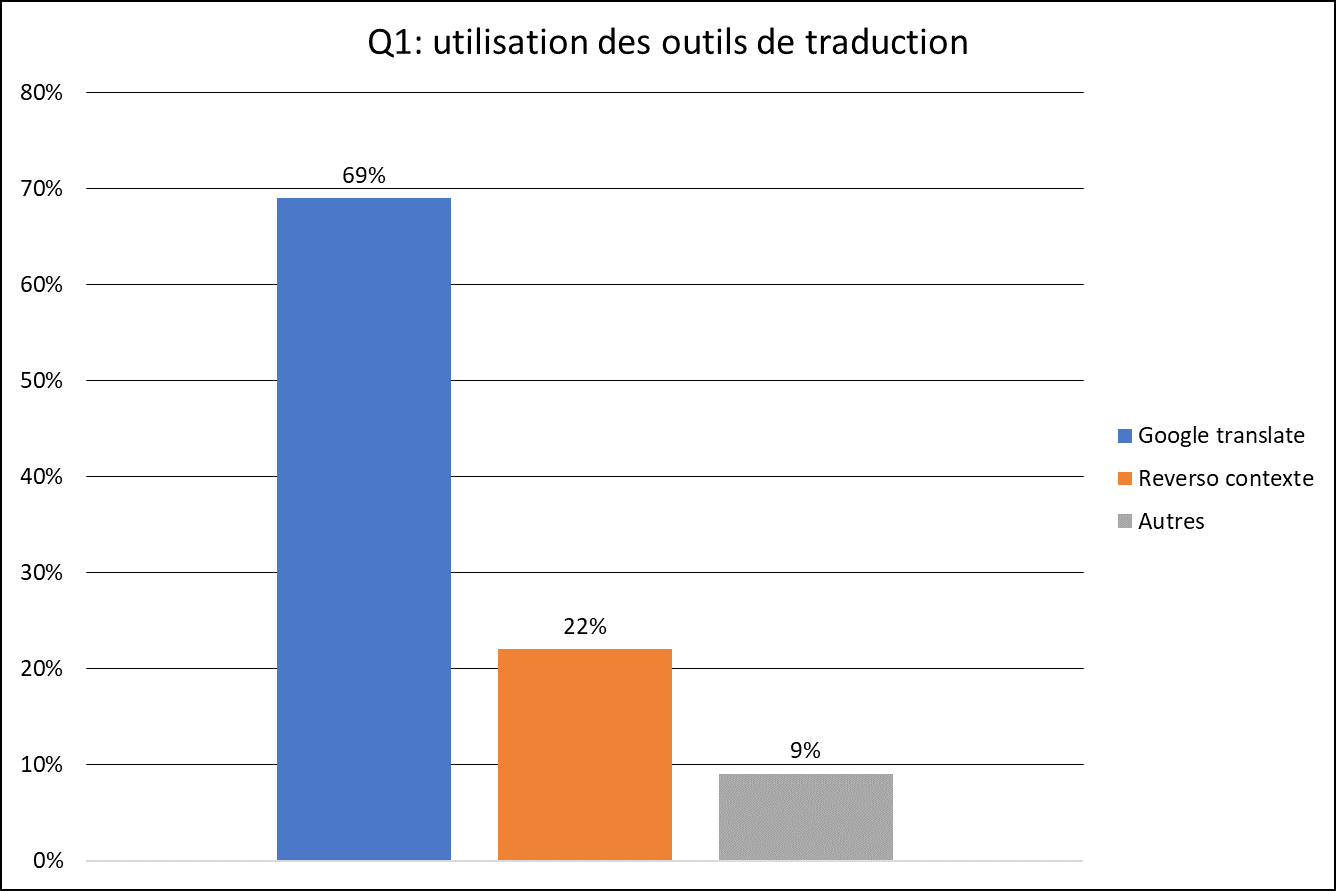
\includegraphics[width=0.85\textwidth]{Fig1.png}
 \caption{Utilisation des outils de traduction.}
 \label{fig1}
 \source{d'après les auteurs.}
\end{figure}

\begin{itemize}
    \item Les outils de traduction dans la traduction des proverbes
\end{itemize}

Les réponses à la deuxième question indiquent que les étudiantes pensent que les outils qui peuvent être utilisés dans la traduction des proverbes sont \textit{Google Translate}, 
\textit{Reverso Contexte}, le dictionnaire Al Maany" et les moteurs de recherche.  La majorité des étudiantes (63\%) voit que \textit{Google Translate} est le moyen qui peut être utilisé pour traduire les proverbes. D’autres voient que la traduction des proverbes est possible quand ils utilisent les dictionnaires bilingues Al Maany (22\%), 
\textit{Reverso Contexte} (13\%) et les outils de recherche (3\%). Pour cette dernière catégorie, les étudiantes disent qu’il n’existe pas d’excellent outil pour traduire le proverbe car il faut rechercher son équivalent dans la langue cible (\Cref{fig2}). 

\begin{figure}[htbp]
 \centering
 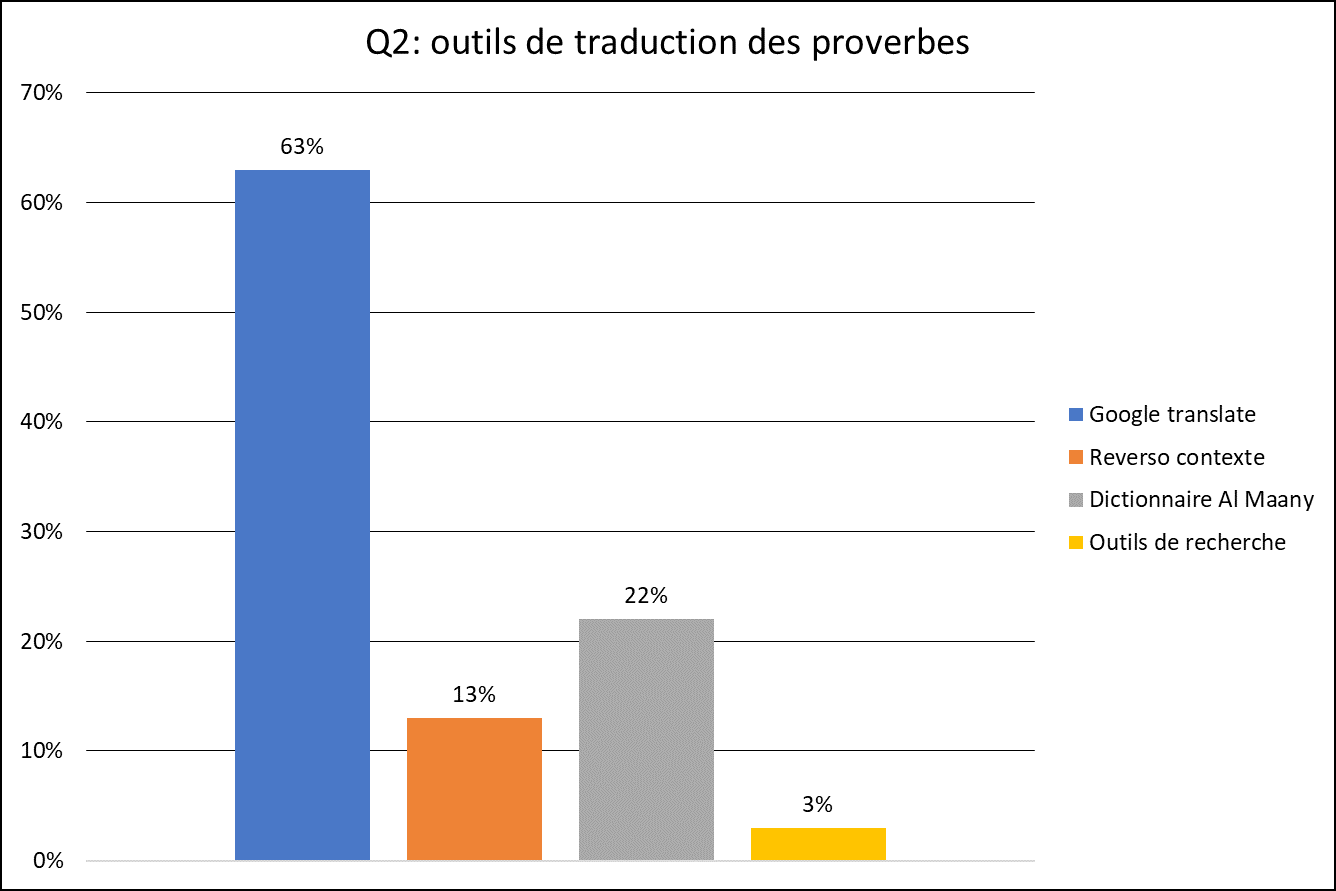
\includegraphics[width=0.85\textwidth]{Fig2.png}
 \caption{Utilisation des outils de traduction dans la traduction des proverbes.}
 \label{fig2}
 \source{d'après les auteurs.}
\end{figure}

\subsection{Traduction des proverbes par l’utilisation de \textit{Google Translate}}\label{sec-modelo}
Les traductions données par \textit{Google Translate} sont présentées dans le \Cref{tbl02}. Nous les avons collectées dans des fiches distribuées aux étudiantes pour faire la traduction. Différentes traductions ont été notées pour un même proverbe bien que toutes les étudiantes aient utilisé le même moteur de traduction. Les traductions arabes ont été jugées incorrectes au niveau sémantique et syntaxique par les étudiantes, qui affirment que les proverbes ont été traduits littéralement sans présenter de proverbe équivalent en arabe, et que la traduction n’évoque absolument rien au lecteur arabe.

\begin{table}[htbp]
\caption{Les différentes traductions des proverbes données par \textit{Google Translate}.}
\label{tbl02}
\begin{tabularx}{\textwidth}{lp{0.44\textwidth}p{0.44\textwidth}}
\toprule
 & Proverbes & Google Translate \\
\midrule
1 & Quand on parle du loup, on en voit la queue &  
\textlang{arabic}{عندما نتحدث عن الذئب، نرى الذيل}\newline
ndama natahadth 'n adh'b, nara adhail'\newline
\textlang{arabic}{عندما نتكلم عن الشيطان ونحن نرى الذيل}\newline
ndama natakalm 'n ashaitan wa nahno nara adhail'\newline
\textlang{arabic}{عندما نتحدث عن الذئب ونحن نرى الذئب}\newline
ndama natahadth 'n adh'b wa nahno nara adh'b'
\\

2 & Les loups ne se mangent pas entre eux & 
\textlang{arabic}{ذئاب لا تأكل البعض بعض}\newline
dhi'ab la ta'koulou alb'd b'd\newline
\textlang{arabic}{الذئاب لا تأكل بينهما}\newline
Al dhi'ab la ta'koulou bainahouma\newline
\textlang{arabic}{الذئاب لا تأكل بعضها بعضا}\newline
Al dhi'ab la ta'koulou b'douha b'dan
\\

3 & Faire d’une pierre deux coups & 
\textlang{arabic}{ضرب عصفورين بحجر واحد}\newline
Daraba 'ousfourain bi hajaren wahed\newline
\textlang{arabic}{قتل طائرين بحجر واحد}\newline
Qatala tairain bi hajaren wahed\newline
\textlang{arabic}{يقتل طائرين بحجر واحد}\newline
Yaqtoulo tairain bi hajaren wahed\newline
\textlang{arabic}{يصطاد عصفورين بحجر واحد}\newline
Yastado 'ousfourain bi hajaren wahed
\\

4 & Le malheur des uns fait le bonheur des autres & 
\textlang{arabic}{فأن سوء حظ واحد جعل سعادة الاخرين}\newline
Fa'ina sou' haz wahed j'ala sa'dat alakharin\newline
\textlang{arabic}{مصيبة بعض يجعل سعادة الاخرين}\newline
Mousibat b'd yaj'l sa'dat alakharin\newline
\textlang{arabic}{من سوء حظ واحدة جعلت الاخرين سعداء}\newline
'Min sou' haz wahida j'lat alakharin sou'ada\newline
\textlang{arabic}{سوء حظ بعض يجعل سعادة اخرين}\newline
sou' haz b'd yaj'l sa'dat akharin\newline
\textlang{arabic}{فان سوء حظ البعض جعل سعادة الاخرين}\newline
Fa'na sou' haz alb'd j'ala sa'dat alakharin
\\

5 & Après la pluie le beau temps & 
\textlang{arabic}{بعد الأمطار أو أشعة الشمس}\newline
B'd al 'mtar 'w 'shi''at ashams\newline
\textlang{arabic}{بعد العاصفة يأتي المطر}\newline
B'd al 'asifa ya'ti al matar\newline
\textlang{arabic}{وبعد المطر يأتي الطقس الجميل}\newline
Wa B'd al matar ya'ti atqs aljamil
\\

6 & Qui se ressemble s’assemble & 
\textlang{arabic}{من ينظر على حد سواء}\newline
'Mn ynzor 'ala had sawa
\\

7 & L’homme propose, Dieu dispose & 
\textlang{arabic}{يقترح الرجل، الله يتصرف}\newline
Yaqtareh arrajoul, Allah yatasaraf\newline
\textlang{arabic}{الرجل يقترح الله يتصرف}\newline
Arrajoul Yaqtareh, Allah yatasaraf
\\

\bottomrule
\end{tabularx}
\source{d’après l’auteur.}
\end{table}

Pour pouvoir évaluer la traduction automatique des proverbes, nous avons demandé aux étudiantes d’analyser les erreurs de traduction et de les noter sur la fiche d’analyse des erreurs. Nous leur avons également demandé de donner les raisons pour lesquelles elles pensent que les traductions sont erronées.

\section{Analyse des erreurs de la TA des proverbes}\label{sec-organizacao}
Les erreurs syntaxiques ont rapport à l’ordre des mots dans la structure de la phrase en arabe, 
et leur traduction littérale empêche de les faire correspondre aux proverbes équivalents. 
La phrase verbale arabe commence par un verbe, suivi d’un sujet et d’un complément d’objet. 
Par exemple, le proverbe \textit{Après la pluie}, le beau temps est traduit par («\textlang{arabic}{وبعد المطر يأتي الطقس الجميل}») 
(Wa B'd al matar ya'ti atqs aljamil), le verbe \textlang{arabic}{يأتي} ya'ti («venir» ou «arriver») 
n’existe pas dans le proverbe français, mais il est introduit pour respecter les parties constitutives de la phrase verbale en arabe. 
Malgré ce changement dans la phrase arabe, il ne respecte pas l’ordre des mots dans la construction phrastique en arabe car le verbe ne vient pas en premier. 

Quant à la TA littérale, les mots utilisés dans les différentes versions de la traduction automatique 
sont interchangeables dans le proverbe, comme c’est le cas pour le mot \textit{pluie} 
(«\textlang{arabic}{المطر}», al matar), qui change de place dans les différentes traductions, 
se plaçant tantôt au début du proverbe, tantôt à la fin, sans respecter l’ordre des mots dans 
la construction phrastique arabe. Les mêmes remarques sont observées dans la traduction du proverbe 
\textit{l’homme propose, Dieu dispose} («\textlang{arabic}{ـ الرجل يقترح الله يتصرف}», 
Arrajoul Yaqtareh, Allah yatasaraf) où la phrase commence par le sujet et non par le verbe. 

D’autres erreurs syntaxiques concernent l’attribution incorrecte du genre au verbe en arabe quand 
l’accord en genre entre le nom et le verbe est exigé, par exemple dans la traduction \textlang{arabic}{مصيبة بعض يجعل سعادة الاخرين}, 
où le verbe \textlang{arabic}{يجعل} («fait que», yaj'l) n’est pas accordé avec le nom féminin \textlang{arabic}{مصيبة} 
(«catastrophe», Mousibat) mais désigne un nom masculin. L’omission de l’article défini \textlang{arabic}{ال} («les», Al) 
dans la traduction du nom \textit{les loups} («\textlang{arabic}{ذئاب}», dhi'ab) transforme d’ailleurs le nom en nom indéfini.

Les erreurs lexicales figurent parmi les erreurs de la TA. En effet, le choix du lexique en arabe n’est pas 
le même dans toutes les versions de la TA. Dans les différentes traductions arabes du proverbe 
\textit{après la pluie, le beau temps}, \textit{Google Translate} introduit un nouveau lexique tel que 
\textlang{arabic}{أشعة الشمس} («les rayons du soleil», 'shi''at ashams), \textlang{arabic}{العاصفة} 
(«le vent», al 'asifa), qui font partie du champ lexical du mot «temps», mais qui s’éloignent encore de 
la traduction en arabe du sens de la locution proverbiale française.

Les étudiantes ont noté que certaines traductions utilisent une polysémie verbale ou nominale qui donne 
un sens erroné au proverbe en langue cible. Par exemple, dans le proverbe \textit{Faire d’une pierre deux coups}, 
le verbe \textit{faire} est traduit par les verbes \textlang{arabic}{قتل} («a tué», Qatala), \textlang{arabic}{يقتل} («tue», Yaqtoulo,)
et \textlang{arabic}{يصطاد} («chasse», yastado), mais les deux premiers verbes ne peuvent en aucun cas remplacer 
les verbes \textlang{arabic}{أصاب} («a ciblé», Assaba), ou \textlang{arabic}{ضرب} («a battu», Daraba) pour donner 
les proverbes équivalents en arabe («\textlang{arabic}{أصاب عصفورين بحجر واحد}») ou («\textlang{arabic}{ضرب عصفورين بحجر واحد}»). 
Quant au verbe \textlang{arabic}{يصطاد} («chasse», yastado), il donne le même sens du verbe \textlang{arabic}{ضرب} 
(«a battu», Daraba) mais il n’est pas utilisé dans le proverbe en arabe. Pour la polysémie nominale, elle est perçue 
dans l’utilisation de mot \textlang{arabic}{طائرين} («deux oiseaux», Ta'eraen) pour remplacer le mot \textlang{arabic}{عصفورين} 
(«deux oiseaux», 'ousfourain), mais le premier n’est jamais utilisé dans le proverbe arabe bien que son sens soit correct. 
La polysémie nominale est également présentée dans deux autres proverbes: le premier, \textit{le malheur des uns fait le bonheur des autres}, 
où l’utilisation du mot \textlang{arabic}{سوء حظ} («le malheur», sou' hath) se rapproche du sens du mot \textlang{arabic}{مصائب} 
(«catastrophes», massa'bo), mais ne peut en aucun cas le remplacer dans le proverbe. Le deuxième, \textit{l’homme propose, Dieu dispose}, 
où l’utilisation du mot \textlang{arabic}{الرجل} («un individu de sexe masculin», Arrajoul) ne signifie pas \textlang{arabic}{العبد} 
(«un être humain sans précision de sexe, soumis à Dieu», Al abd), qui est le mot utilisé dans locution proverbiale arabe \textlang{arabic}{العبد في التفكير والرب في التدبير}.
 
La traduction littérale donne un sens éloigné des proverbes dans la langue cible ou un faux sens. 
La traduction du proverbe \textit{après la pluie le beau temps} désigne les conditions météorologiques, 
alors que le proverbe en arabe dit que les satisfactions, la gaieté finissent par remplacer les désagréments, 
la tristesse. Quant aux traductions des proverbes qui n’ont pas de sens en arabe, nous donnons comme 
exemple de faux sens, («\textlang{arabic}{الذئاب لا تأكل بينهما}» , Al dhi'ab la ta'koulou bainahouma) 
pour le proverbe \textit{les loups ne se mangent pas entre eux}, et («\textlang{arabic}{من سوء حظ واحدة جعلت الاخرين سعداء}», 
Min sou' haz wahida j'lat alakharin sou'ada') pour le proverbe \textit{le malheur des uns fait le bonheur des autres} 
(«\textlang{arabic}{من ينظر على حد سواء}, Mn ynzor 'ala had sawa') pour \textit{qui se ressemble s’assemble}  et 
(«\textlang{arabic}{عندما نتكلم عن الشيطان ونحن نرى الذيل}», 'ndama natakalm 'n ashaitan wa nahno nara adhail) 
pour \textit{quand on parle du loup, on en voit la queue}.

D’autres proverbes présentent des erreurs stylistiques même si la traduction ne donne pas le proverbe équivalent. 
Par exemple, dans le proverbe \textit{les loups ne se mangent pas entre eux} et traduit 
(«\textlang{arabic}{ذئاب لا تأكل البعض بعض}» , dhi'ab la ta'koulou alb'd b'd), le pronom «se» et le complément «entre eux» 
sont traduits par («\textlang{arabic}{البعض بعض}», alb'd b'd). Cela n’est pas acceptable en arabe du fait de la répétition 
de mots qui ne sont pas reliés par une particule («\textlang{arabic}{ها}» ha (quelqu’un), ce qui produit une expression 
sans aucun sens. Il est à signaler que certaines propositions de traduction automatique étaient correctes pour les deux 
proverbes français \textit{les loups ne se mangent pas entre eux} et \textit{faire d’une pierre deux coups}.

Les erreurs montrent que le logiciel de traduction automatique offre des performances peu satisfaisantes au niveau de 
la traduction des proverbes et de la qualité générale des traductions obtenues tant sur le plan syntaxique, lexical et sémantique que stylistique. 

\section{La Post-édition de la TA des proverbes}\label{sec-organizacao-latex}
Les étudiantes ont mis en place plusieurs stratégies pour trouver l’équivalent du proverbe en arabe et pour vérifier que le proverbe correspond à des normes satisfaisantes en langue cible. Parmi ces stratégies qui varient en fonction des problèmes de TA pour chaque proverbe, évoquons les suivantes :

\begin{itemize}
    \item \textbf{Après la pluie le beau temps}
    \item Décomposition du proverbe en mots et la recherche du sens des mots séparés dans les dictionnaires en ligne, comme le dictionnaire \textit{reverso.com}.
    \item Compréhension du sens des mots et la déduction du proverbe arabe qui pourrait donner le même sens ainsi que la recherche documentaire pour vérifier si le proverbe déduit est équivalent au français.
    \item Recherche sur Google du proverbe équivalent en anglais ayant le même sens que le proverbe traduit.
    \item \textbf{Qui se ressemble s’assemble, les loups ne se mangent pas entre eux, faire d’une pierre deux coups}
   \item Utilisation du moteur de traduction du dictionnaire \textit{reverso.com} pour chercher la traduction du proverbe du français en arabe.
   \item Recours aux connaissances antérieures des proverbes dans la langue maternelle des étudiantes et le jugement subjectif sur l’adéquation de la traduction de ce proverbe. 
   \item Recherche sur plusieurs sites internet de l’équivalent arabe des proverbes.
   \item Recherche documentaire sur les expressions figées en arabe utilisant un mot du proverbe, comme « les loups ». Cette stratégie a conduit à avoir un équivalent sous une autre forme, à savoir un vers d’une poésie d’Al-Imam Al Shafe'e («\textlang{arabic}{وَلَيسَ الذِئبُ يَأكُلُ لَحمَ ذِئبٍ}» wa layssa al dh'bo ya'koulo dh'ban),  ce qui signifie un loup ne mange pas la chair d’un autre loup.
   \item \textbf{Le malheur des uns fait le bonheur des autres}
   \item Consultation de la traduction du proverbe en langue cible dans le dictionnaire \textit{reverso.com}, où il est mentionné.
   \item \textbf{L’homme propose, Dieu dispose}
   \item Traduction du sens général du proverbe en langue-source pour présenter un sens du proverbe sémantiquement proche de celui en 
   langue-cible sans recourir à la traduction littérale («\textlang{arabic}{قضاء الله قادم مهما حلم العبد}»).
   \item Compréhension du sens général de l’expression proverbiale par la recherche de son origine. L’idée de l’expression vient de la Bible et elle représente la providence divine exercée sur le monde par Dieu. Les étudiantes ont déduit le verset équivalent du sens du proverbe (numéro 29) dans le Coran, sourate 81- At-Takwir (l’obscurcissement) 
   («\textlang{arabic}{وَمَا تَشَاءُونَ إِلا أَنْ يَشَاءَ اللَّهُ رَبُّ الْعَالَمِين}», wa ma tashaouna 'lla an yasha'a Allaho rab el alameen), ce qui est traduit par 
   («Mais vous ne pouvez vouloir, que si Allah veut, [Lui], le Seigneur de l’Univers»)\footnote{\url{https://surahquran.com/translation/frinsh/586.html}}.
   \item \textbf{Quand on parle du loup, on en voit la queue}
   \item Recherche du sens du proverbe français dans le dictionnaire en ligne \textit{larousse.fr}.
   \item Division du proverbe en deux parties syntaxiques et traduction de chaque partie indépendamment de l’autre.
   \item Recherche du sens de chaque partie en anglais.
   \item Traduction du proverbe en langue-cible familière après la compréhension de son sens en anglais.
   \item Recherche du proverbe équivalent en arabe dans les références documentaires et les ouvrages des proverbes français comme le dictionnaire bilingue des proverbes français.
\end{itemize}

\section{Discussion}\label{sec-autores}
Les résultats du questionnaire montrent que la majorité des étudiantes utilisent \textit{Google Translate} 
pour la traduction générale des textes. D’autres outils sont utilisés, comme les dictionnaires en ligne tels 
que \textit{Reverso Contexte} et le dictionnaire bilingue arabe-français / français-arabe Al Maany. 
En effet, les étudiantes préfèrent utiliser \textit{Google Translate} également pour la traduction des proverbes. 
Pourtant, selon les réponses des étudiantes, le taux d’utilisation des autres outils de traduction automatique tels 
que \textit{Reverso Contexte} et le dictionnaire bilingue Al Maany varient selon le type de traduction. 
Quand la traduction est générale, les étudiantes utilisent \textit{Reverso Contexte} plus que le dictionnaire Al Maany, 
mais ce dernier est censé être plus utilisé quand il s’agit de la traduction des proverbes. 

Les étudiantes qui pensent que les outils de recherche sont les outils les plus adaptés pour chercher l’équivalent 
des proverbes en arabe sont moins nombreuses. Ces résultats montrent généralement que la majorité des étudiantes ne 
connaissent pas les limites de l’outil \textit{Google Translate} pour les proverbes, ce qui nous a incité à commencer par 
leur formation aux limites de l’outil non seulement au niveau de la traduction des expressions générales mais aussi 
au niveau de la traduction des proverbes français. En effet, comme nous l’avons évoqué dans la partie théorique, les 
spécificités de la traduction des proverbes retiennent une attention particulière de la part du traducteur, et il en 
est de même pour la traduction par la machine. Les structures syntaxiques, le choix du lexique et la sémantique du 
proverbe devraient être pris en compte dans la traduction.

L’objectif de l’analyse des erreurs de traduction et de post-édition des proverbes est de montrer aux apprenties 
traductrices que les questions de traduction de la sémantique continuent bien évidemment de se poser, en dépit 
des développements technologiques récents pour ne pas récolter les «fruits les plus faciles à atteindre» dans 
la traduction automatique \cite{poibeau_traduire_2016}, notamment celle des expressions figées. En effet, la 
post-édition des proverbes français par les apprenties traductrices a été abordée en tant que problème à résoudre, 
une notion qui prend de plus en plus d’importance dans le domaine de la traduction, dans la mesure où elles n’ont 
pas eu suffisamment de connaissances sur le sens des expressions figées en français malgré leur fréquence en langue, 
et où le proverbe a déclenché dans sa traduction une série de processus mentaux \cite{gil-bardaji_resolution_2010}. 
Le fait de permettre aux étudiantes d’expérimenter la traduction automatique des proverbes a permis de les sensibiliser 
aux erreurs commises et de corriger les textes traduits en adoptant des stratégies variées, auxquelles l’enseignante 
ne pense même pas forcément spontanément dans un premier temps.

Les erreurs ont été classifiées en fonction des résultats et non selon des catégories préétablies. Cette classification 
peut en fait constituer une base d’élaboration pour une typologie des erreurs de la traduction automatique des proverbes 
dans la paire de langues français-arabe, qui à notre connaissance n’existe pas au moment où nous écrivons ces lignes. 
Cette typologie est constituée de quatre catégories essentielles:

\begin{itemize}
    \item Les erreurs sémantiques: la polysémie verbale ou nominale, le faux-sens, la traduction littérale menant au non-sens.
    \item Les erreurs syntaxiques: la construction phrastique en arabe, l’ordre incorrecte des mots dans la phrase, l’omission de l’article défini, l’interchangeabilité des mots de la phrase, l’absence d’accord du genre et du nombre entre les différentes unités de la phrase (nom et verbe).
    \item Les erreurs lexicales: introduction du nouveau lexique sans ajouter de valeur sémantique au proverbe, traduction incorrecte du lexique.
    \item Les erreurs stylistiques: répétition des mots.
\end{itemize}

Bien que les erreurs montrent l’insuffisance de la performance de la traduction pour cinq proverbes, la traduction automatique était correcte pour deux d’entre eux, et ce résultat contredit l’idée de l’incapacité de la TA à traduire les proverbes français en arabe. Mais, Il est aussi possible que les deux proverbes traduits correctement ont été suggéré par quelqu’un qui connait les deux langues.

Il est important de préciser que même pour les cinq proverbes qui n’ont pas été traduits correctement,  
les versions proposées par \textit{Google Translate} ont permis aux étudiantes d’établir des rapprochements syntaxiques 
et sémantiques entre les deux paires de langues pour pouvoir comprendre leur sens avant de rechercher leur équivalent, 
soit avec l’introduction du verbe \textlang{arabic}{يأتي} («venir» ou «arriver», ya'ti ), ou avec une proposition dans 
la TA de mot qui n’existait pas dans le proverbe français \textlang{arabic}{عصفورين} («deux oiseaux», 'ousfourain). 
Ces propositions de traductions ont aidé les étudiantes à déduire l’expression équivalente en arabe, ce qui permet 
d’élargir l’expérience des étudiantes dans la post-édition des proverbes et de développer des compétences transversales 
pour la post-édition d’autres textes comprenant des phénomènes linguistiques, sémantiques et métaphoriques. L’effet positif de ce type d’expérience de la post-édition est, en définitive, le changement d’attitude des étudiants, qui développement une vision plus positive de la TA \cite[p.~13]{koponen_how_2015}.

Les étudiantes ont de toute façon mis en œuvre différentes stratégies dans la post-édition afin de corriger la TA proposée. 
Ces stratégies varient en fonction du niveau linguistique des étudiantes (débutant ou intermédiaire), de leur compréhension 
des expressions proverbiales et de leur capacité à établir des liens entre ces expressions et celles de leur langue maternelle. 
Au niveau linguistique, elles ont procédé au découpage des proverbes à traduire en exploitant le sens donné par \textit{Google Translate} 
à ces unités. Par exemple le mot \textit{Pluie} correspond au sens dénotatif en arabe (« matar ») dans le proverbe \textit{Après la pluie le beau temps}. 
L’outil de la TA a constitué une aide immédiate dans cette stratégie qui est identique au processus de traitement automatique des 
langues évoqué par \textcite{bessou_contribution_2019} lors du travail sur la paire de langues anglais-arabe.

Les processus adoptés par les étudiantes dans la post-édition passent par des choix stratégiques éclairants puisque que la traduction proverbiale automatique n’était pas considérée comme fiable. Ces stratégies ont été organisées de manière à viser la recherche du sens des proverbes (voir \Cref{fig1}). La décomposition des proverbes en mots et en unités lexicales a aidé les étudiantes à trouver leur sens et à réfléchir sur leur relation avec le sens des proverbes en arabe.

Lorsque cette première stratégie n’a pas produit de sens différent du celui du proverbe donné par \textit{Google Translate}, les étudiantes ont recherché le sens du proverbe complet sur des sites internet et dans les dictionnaires en ligne. Cette deuxième stratégie vise la recherche du sens dans les unités phrastiques et non pas dans l’équivalence lexicale des mots puisque la traduction proverbiale doit avoir une équivalence sémantique de l’ensemble du groupe. La correction des structures formelles des proverbes traduits automatiquement n’a pas constitué l’étape principale dans la post-édition.

La troisième stratégie était l’utilisation de la langue anglaise comme langue-pivot. Une fois le proverbe est connu en anglais, son sens devient plus facile à reconnaitre en arabe. La quatrième stratégie constituait à dire le proverbe en arabe familier, ou bien son équivalent sous d’autres formes, comme un vers de poème ou un verset du Coran. En fait, le recours à la citation des versets du Coran ou des Hadiths contenant des expressions figées est une pratique récurrente chez les chercheurs lors de leur comparaison dans deux langues, l’arabe et l’anglais \cite[p.~83]{alhomoud_articulation_2020} ou le français, car ils constituent des ressources riches en métaphores ou proverbes qui représentent la culture arabe. De plus, la quatrième stratégie sensibilise les étudiantes à la variété des ressources et des options de solutions de problèmes dans la traduction.

Enfin, la dernière stratégie était la recherche documentaire dans les livres de référence en arabe sur le proverbe équivalent en arabe standard. En dernier recours, la validation ou la non-validation de la traduction des proverbes est une décision de l’enseignante (\Cref{fig3}).

\begin{figure}[htbp]
 \centering
 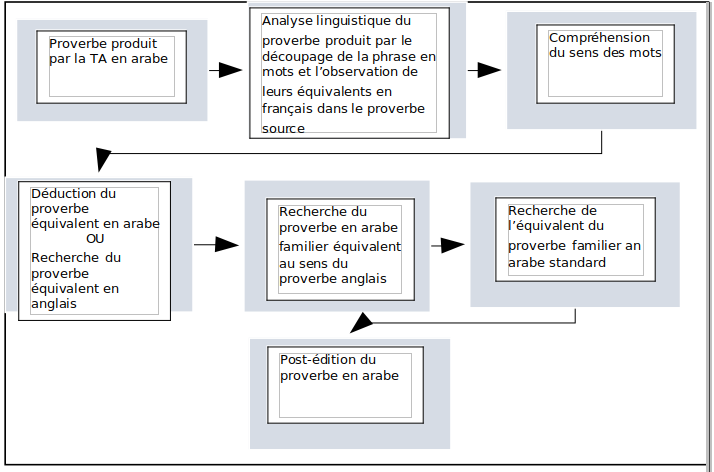
\includegraphics[width=0.85\textwidth]{Fig3.png}
 \caption{Organisation des stratégies selon les étapes de la post-édition.}
 \label{fig3}
 \source{d'après les auteurs.}
\end{figure}

Une réflexion didactique sur les différentes stratégies mises en œuvre nous conduit à dire qu’elles ont visé la forme sémantique des proverbes en langue-cible et ne sont pas seulement centrées sur la recherche de l’équivalent lexical des mots. Cela explique une prise en compte par les étudiantes de l’ensemble des mots qui définissent leur signification \cite{elouafa_proverbe_2015}. De plus, la complexité de la traduction de certains proverbes les a conduites à réfléchir à plusieurs stratégies et à mobiliser plus de processus cognitifs, voire à recourir à des stratégies créatrices capables de résoudre un problème \cite[p.~285]{gil-bardaji_resolution_2010} dans la post-édition des proverbes, qui peut être considérée comme un problème qui n’a pas de solution prédéterminée.

Le recours à une langue-pivot comme l’anglais est légitime dans la mesure où il permet de trouver un proverbe équivalent qui crée le cadre d’une analogie que le locuteur utilise pour légitimer une opinion \cite[p.~64]{milica_proverbes_2013}. Notons que l’anglais est la première langue étrangère apprise par les étudiantes (L2 dans l’acquisition des langues) après l’arabe (L1) et avant l’apprentissage du FLE (L3), il est donc normal de recourir à L2 pour chercher des repères sémantiques afin de faciliter la post-édition.

\section{Conclusion}\label{sec-idioma}
Dans le cadre de cette recherche, nous avons essayé d’identifier les stratégies mises en œuvre dans la résolution de problèmes de traduction de proverbes produite par les outils de traduction en ligne. Notre réflexion didactique sur l’importance de ces stratégies dans la formation réflexive de futures traductrices va dans le sens du développement des compétences des apprenties traductrices. Leur sensibilisation aux erreurs de traduction automatique des proverbes permet de les rendre plus attentives au sens de ces derniers et à leur réception selon les cultures des langues concernées. Certes, les étudiantes ont commencé à acquérir ces stratégies grâce à la pratique et à l’entrainement ; mais nous avons également mis en exergue au cours de ce travail les caractéristiques de ces stratégies, en définissant également leur organisation dans le processus général de post-édition, ce qui nous permettra d’agir directement sur la méthodologie de la traduction des proverbes et sur la formation à la post-édition pour la paire de langues français-arabe. 

Une étude plus développée avec un nombre important de proverbes devrait cependant être menée afin de développer la typologie des erreurs et d’identifier d’autres stratégies de post-édition fructueuses pour la formation de futures traductrices. Il serait également intéressant de voir si des étudiantes à un niveau linguistique plus avancé utilisent d'autres outils de traduction automatique et de mener d’autres expériences pratiques pour vérifier si ces outils donnent les mêmes résultats que \textit{Google Translate}. Ainsi, nous pourrions procéder à l’identification de stratégies de post-édition mises en œuvre avec ces autres outils, car l’apport de départ avant le processus de la post-édition pourrait bien varier en fonction de l’outil de traduction automatique.

\section{Acknowledgment}\label{sec-resumo}
This research was funded by the Deanship of Scientific Research at Princess Nourah Bint Abdulrahman University through the Fast-track Research Funding Program.

\printbibliography\label{sec-bib}
% if the text is not in Portuguese, it might be necessary to use the code below instead to print the correct ABNT abbreviations [s.n.], [s.l.] 
%\begin{portuguese}
%\printbibliography[title={Bibliography}]
%\end{portuguese}

\end{document}
